\chapter{Security}

As the main goal of our whole architecture is to extract information and actionable insights from data, there needs to be a tight security customized to our infrastructure in order to protect that valuable data.
To protect the data we use several layers of security, some seen commonly in other systems, some peculiar to our stack.
\newline
Firstly, access to the cluster internal network must be denied to every outside request but for few selected ports on a front end machine, this is obtained through standard ACLs.
The only connections available to both Clients and Developers must be through secure channels (HTTPS\footnote{HTTPS: HyperText Transfer Protocol over Secure Socket Layer, standard protocol for secure web pages}, SSH\footnote{SSH: Secure SHell, protocol for remote controls of Command Line Interfaces}, FTPS\footnote{FTPS: File Transfer Protocol over Secure Socket Layer, self explanatory}).
\newline
Secondly, the author of the request that passed through ACL must be authenticated by an authentication provider such as LDAP\footnote{LDAP: Lightweight Directory Access Protocol, a standard protocol  for accessing distributed directory information services over an intranet} or Kerberos, and then authorised to follow through with its request with respect to its identity.
\newline
Thirdly, a service must provide Auditing for all requests, whether denied or allowed so that actions and their consequences can be attributed to their authors.

\pagebreak

\section{Knox}

\textbf{Apache Knox} \cite{knox_doc} is an Application Gateway, part of the Hadoop environment, that offers several security functionalities for a Hadoop Cluster right after the first layer provided by the ACL and acts as a Reverse Proxy with policy enforcement.
\subsection{Authentication and Acces Control}
The Knox gateway exposes a single secure access point for all REST\footnote{REST: REpresentational State Transfer, a type of stateless software architecture whose aim is to provide access to resource in an interoperable way through the web} APIs and HTTP interactions with the cluster.\newline
All client requests to RESTful APIs and webUIs are sent to Knox through HTTPS with their respective user credentials, Knox authenticates the user with the help of an authentication provider such as Kerberos or LDAP, then thanks to an authorisation provider offers Access Control to the single services, if access is allowed, the request is routed to the target service.
Failed authentication, failed authorisation and successful requests are all logged, providing a first layer of Auditing.
\pagebreak

\subsection{Structure}
The two main components of Knox are the Topology files and the services' files.
\newline
The Topology is an XML file representing a gateway, it is divided in two main sections: the gateway/provider section and the service section; the former section is comprised of the configuration settings enforced by the gateway while providing access to the Hadoop cluster, these settings describe the services that fulfil various roles such as the Authentication provider, the Federation or Single Sign-On provider, the Authorisation provider and the Hostmap which maps external to internal node hostnames.
The service section provides a list of services accessible from the gateway and the address in the cluster where they can be found.
\newline
For each service listed in the Topology, two files are needed: 
\begin{itemize}
	\item service.xml, which defines the high level URL patterns to be exposed by the gateway for that service, such as the shape of the incoming request to be matched.
	\item rewrite.xml, which defines regular expression through which the request must be rewritten before being sent to the cluster internal service.
\end{itemize}
Knox comes packaged with several files for common Hadoop services and permits the definition of custom ones. 

\section{Ranger}

\textbf{Apache Ranger} \cite{ranger_doc} is a comprehensive framework to manage data security, authorisation, data governance and audit in Hadoop clusters.

Ranger provides a centralised security administration able to manage in one place most of the security related tasks inside the cluster, with a high granularity thanks to its customization for Hadoop services.

Plain authentication is accepted, and can be used if a previous layer has already authenticated the user (such as Knox), otherwise Ranger supports LDAP and Unix Authentication.

\subsection{Authorisation}
A request coming from within the cluster to a service for which Ranger is enabled, provided previous authentication, must be authorised by Ranger according to precise policies specific to the service.

Ranger supports several plugins for the major services containing critical data, such as HDFS, HBase, Hive and YARN plus a selection of other services that process or ingest data and interact with the former four.
\newline Authorization can be granted through policies to certain groups or users to services altogether (access-authorization) or to specific resources inside them (resource-classification).
\newline
To exemplify the granularity provided by Ranger, here's presented an image depicting a policy on Hive that allows only \textbf{SELECT} requests from a restricted group on certain rows of a specific table in a database.

\begin{figure}
	\centering
	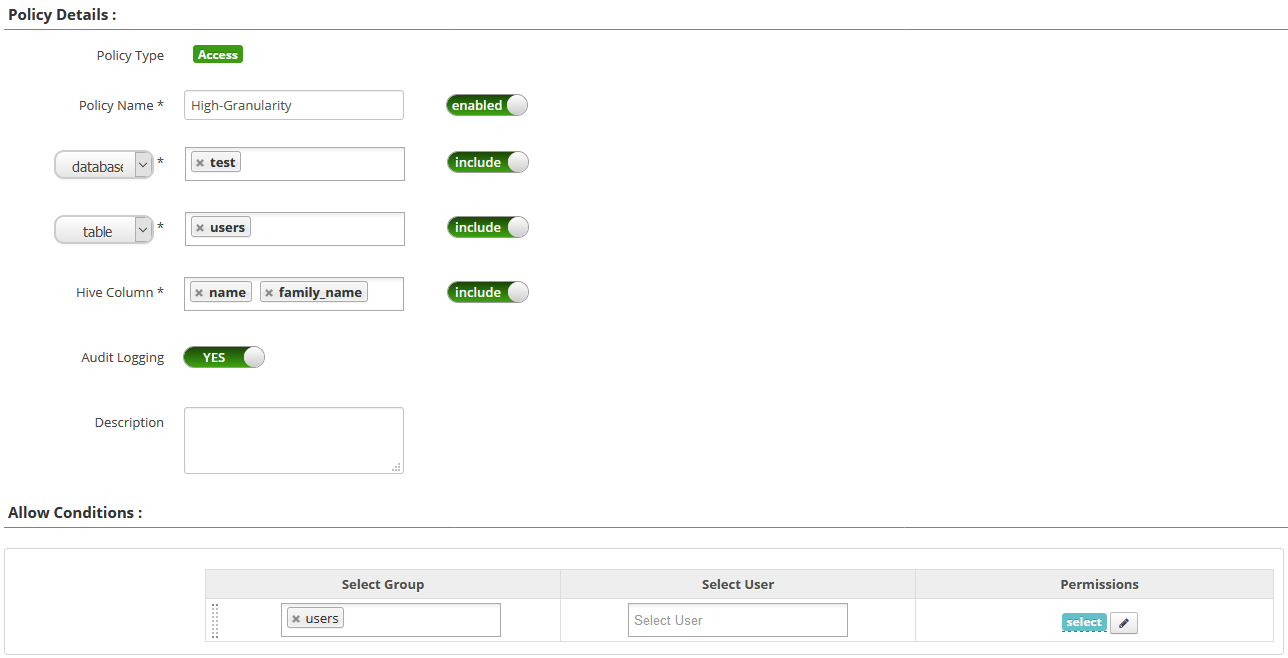
\includegraphics[scale=0.4]{Figures/policy.png}
	\decoRule
	\caption[Infrastructural Stack]{A Ranger policy for Hive}
	\label{fig:Policy}
\end{figure}

\subsection{Tag Based Policies and Persistence}

New versions of Ranger support a new type of Policy based on Tags; Tags can be associated with single resources inside other services, providing those resources the same kind of policy without having to specify it, this makes it easier to separate access-authorization and resource-classification and to manage the latter.\newline
Tags and related information are stored in the Tag Store, while a TagSync process is responsible for synchronisation with other services using Tags such as Apache Atlas.
\newline
Policies and users are stored in a MySQL database on one of the hosts' file system, a synchronisation process is designated with managing users between Ranger, Ambari and other security services such as LDAP/Active Directory.\newline
Auditing of all accesses are stored on HDFS directly or through Apache Solr, a fast search engine.